\documentclass{article}

\usepackage{graphicx}
\usepackage{amsmath}
\usepackage{amssymb}
\usepackage{gensymb}

\begin{document}

\title{Documentation de la suite logicielle GBMProject3A}
\author{Guillaume Gibert}
\maketitle

%%%SECTION%%%%%%%%%%%%
\section{Introduction}
Ce document décrit les différents éléments de la suite logicielle GBMProject3A.

\subsection{Côté PC}
Le code fourni est écrit en C++ avec comme unique dépendance l'API Qt.
Il se compose d'un ensemble de classes qui permettent:
\begin{itemize}
\item de communiquer avec un système Arduino que ce soit en réception ou en émission;
\item de traiter des signaux (filtrage, FFT);
\item d'afficher des signaux;
\item de faire des requêtes sur une base de données MySQL.
\end{itemize}

\subsection{Côté Arduino}
Un code de test est fourni qui permet d'envoyer sous forme de chaîne de caractères standardisée les valeurs lues sur les 5 canaux analogiques de la carte Arduino. Une fonction de lecture d'évènements est également mise en place pour lire, en parallèle, les données sur le port série provenant du PC.


Une série d'exemples permet d'implémenter chaque fonctionnalité. Ils vont être décrit dans la suite du document.

%%%SECTION%%%%%%%%%%%%
\begin{figure}
 \centering
    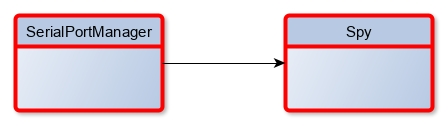
\includegraphics[width=10cm]{images/GBMProject3A_ex1.jpg}
    \caption{Les données de l'Arduino sont captées par l'objet SerialPortManager qui les envoie à l'objet Spy.}
    \label{ex1}
\end{figure}

\section{Exemple 1: Récupérer des données depuis un Arduino (liaison filaire)}
Dans cet exemple, deux objets sont instantiés (voir Figure~\ref{ex1}). Un objet de type SerialPortManager récupère les données envoyées par l'Arduino sur le port série. 
Il envoie ensuite, via un signal/slot Qt, les données vers un objet de type Spy qui les affiche à l'écran.


%%%SECTION%%%%%%%%%%%%
%\begin{figure}
% \centering
%    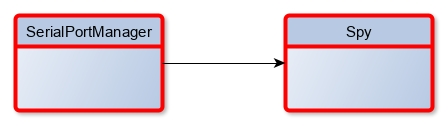
\includegraphics[width=10cm]{images/GBMProject3A_ex2.jpg}
%    \caption{Les données de l'Arduino sont captées par l'objet SerialPortManager qui les envoie à l'objet Spy.}
%    \label{ex2}
%\end{figure}

\section{Exemple 2: Récupérer des données depuis un Arduino (liaison Bluetooth)}

Cet exemple est similaire au précédent (cf. Figure~\ref{ex1}). La seule différence réside dans le type de connexion entre l'Arduino et le PC. 
Dans l'exemple précédent, L'Arduino était connecté avec un cable USB au PC alors que dans cet exemple, il est connecté en Bluetooth via un module HC-05 par exemple.

%%%SECTION%%%%%%%%%%%%
\section{Exemple 3: Récupérer des données depuis un générateur de signaux}

%%%SECTION%%%%%%%%%%%%
\section{Exemple 4: Afficher des signaux temporels}

%%%SECTION%%%%%%%%%%%%
\section{Exemple 5: Filtrer des signaux temporels}


%%%SECTION%%%%%%%%%%%%
\section{Exemple 6: Calculer une transformée de Fourier rapide (FFT)}


%%%SECTION%%%%%%%%%%%%
\section{Exemple 7:  Envoyer une chaîne de caractères à l'Arduino}

%%%SECTION%%%%%%%%%%%%
\section{Exemple 8:  Gérer une base de données "patient" depuis une interface graphique}

\end{document}